\documentclass[a4paper, 14pt]{extarticle}
\usepackage[russian]{babel}
\usepackage[T1]{fontenc}
\usepackage{fontspec}
\usepackage{indentfirst}
\usepackage{enumitem}
\usepackage{graphicx}
\usepackage[
  left=20mm,
  right=10mm,
  top=20mm,
  bottom=20mm
]{geometry}
\usepackage{parskip}
\usepackage{titlesec}
\usepackage{xurl}
\usepackage{hyperref}
\usepackage{float}
\usepackage[
  figurename=Рисунок,
  labelsep=endash,
]{caption}
\usepackage[outputdir=build, newfloat]{minted}

\hypersetup{
  colorlinks=true,
  linkcolor=black,
  filecolor=blue,
  urlcolor=blue,
}

\renewcommand*{\labelitemi}{---}
\setmainfont{Times New Roman}
\setmonofont{JetBrains Mono}[
  SizeFeatures={Size=11},
]

\newenvironment{code}{\captionsetup{type=listing}}{}
\SetupFloatingEnvironment{listing}{name=Листинг}

\setminted{
  fontsize=\footnotesize,
  frame=lines,
  framesep=2mm,
}

\setlength{\parskip}{6pt}

\setlength{\parindent}{1cm}
\setlist[itemize]{itemsep=0em,topsep=0em,parsep=0em,partopsep=0em,leftmargin=2.0cm,wide}
\setlist[enumerate]{itemsep=0em,topsep=0em,parsep=0em,partopsep=0em,leftmargin=2.0cm,wide}

\renewcommand{\thesection}{\arabic{section}.}
\renewcommand{\thesubsection}{\thesection\arabic{subsection}.}
\renewcommand{\thesubsubsection}{\thesubsection\arabic{subsubsection}.}

\titleformat{\section}{\normalfont\bfseries}{\thesection}{0.5em}{}
\titleformat{\subsection}{\normalfont\bfseries}{\thesubsection}{0.5em}{}

\titleformat*{\section}{\normalfont\bfseries}
\titleformat*{\subsection}{\normalfont\bfseries}

\linespread{1.5}
\renewcommand{\baselinestretch}{1.5}

\begin{document}

\begin{titlepage}
  \vspace{0pt plus2fill}
  \noindent

  \vspace{0pt plus6fill}
  \begin{center}
    Санкт-Петербургский национальный исследовательский университет
    информационных технологий, механики и оптики

    \vspace{0pt plus3fill}

    Факультет инфокоммуникационных технологий

    Направление подготовки 11.03.02

    \vspace{0pt plus2fill}

    Лабораторная работа №2
  \end{center}

  \vspace{0pt plus6fill}
  \begin{flushright}
    Выполнил: \\
    Швалов Даниил Андреевич

    Группа: К33211

    Проверила: \\
    Марченко Елена Вадимовна
  \end{flushright}

  \vspace{0pt plus5fill}
  \begin{center}
    Санкт-Петербург

    2024
  \end{center}
\end{titlepage}

\section{Введение}

\textbf{Цель работы}: разработать программу (с использованием средства
разработки VBA и Delphi) с удобным графическим интерфейсов для нахождения корня
уравнения с заданной степенью точности методом деления отрезка пополам.

\section{Ход работы}

\subsection{Разработка с помощью VBA}

Для разработки программы на языке программирования Visual Basic была выбрана
среда разработки Visual Studio 2022, поскольку она обладает обширным
инструментарием для создания программ с графическим интерфейсом на данном языке
программирования.

На рисунке \ref{fig:vba/design} показан дизайн приложения, который был
сделан с помощью средств разработки интерфейсов Visual Studio 2022. В нем есть
поля для ввода границ интервалов, а также точности (эпсилон).

\begin{figure}[H]
  \centering
  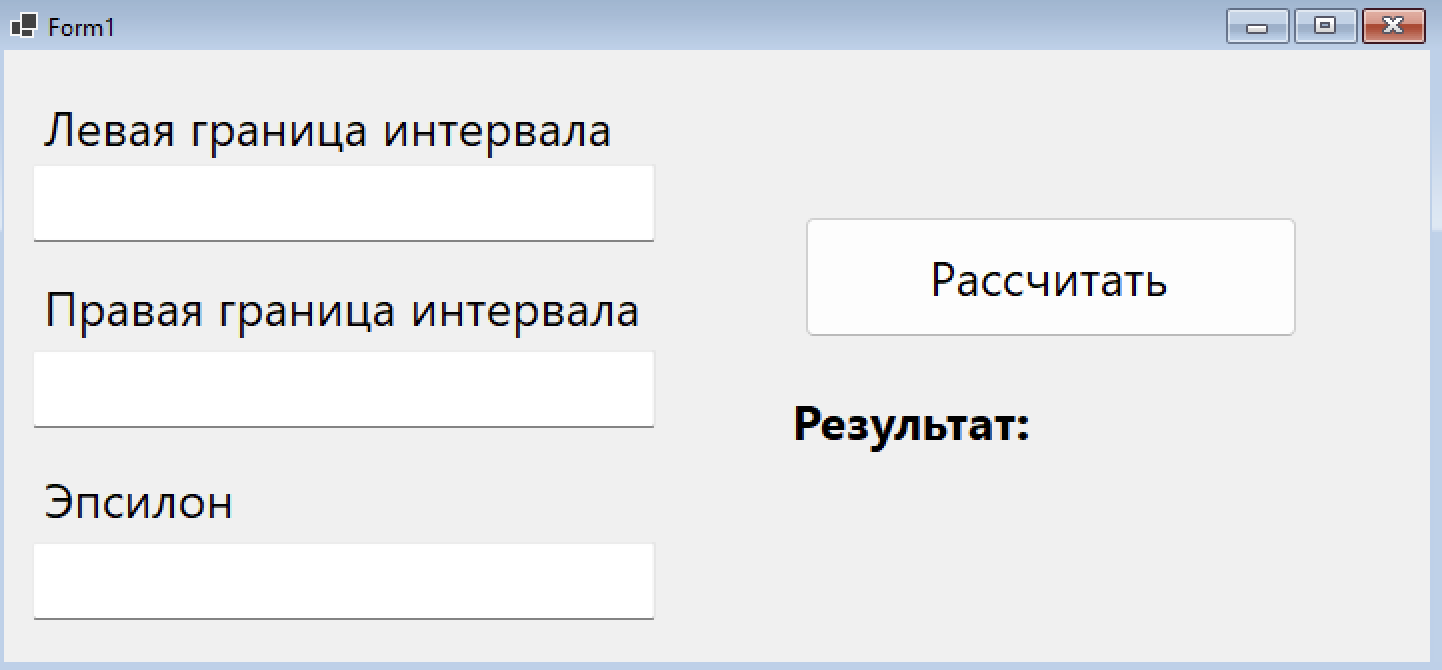
\includegraphics[width=0.7\textwidth]{images/vba/design.png}
  \caption{Дизайн приложения для вычисления корня уравнения}
  \label{fig:vba/design}
\end{figure}

При запуске программы открывается окно, показанное на рисунке
\ref{fig:vba/empty-form}. После ввода данных и нажатия на кнопку <<Рассчитать>>,
как показано на рисунке \ref{fig:vba/filled-form}, рядом с надписью
<<Результат>> появилось вычисленное значение корня уравнения.

\begin{figure}[H]
  \centering
  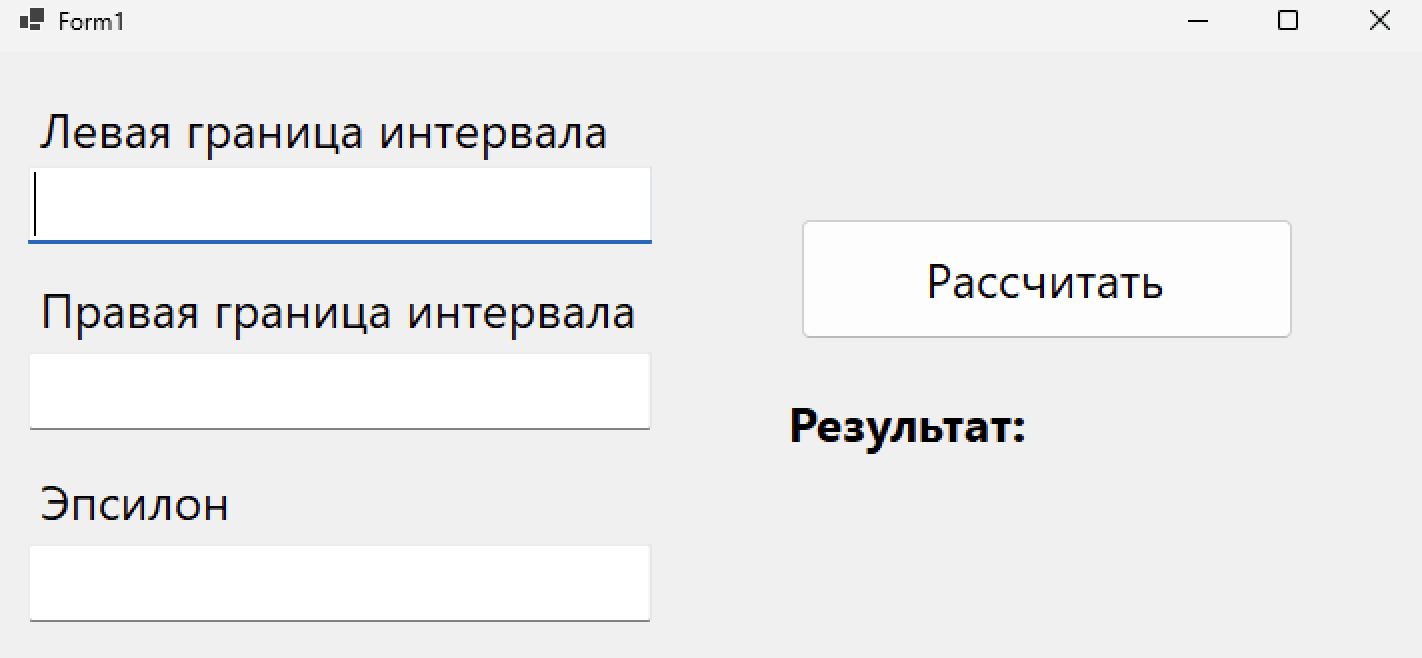
\includegraphics[width=0.7\textwidth]{images/vba/empty-form.png}
  \caption{Приложение для вычисления корня уравнения}
  \label{fig:vba/empty-form}
\end{figure}

\begin{figure}[H]
  \centering
  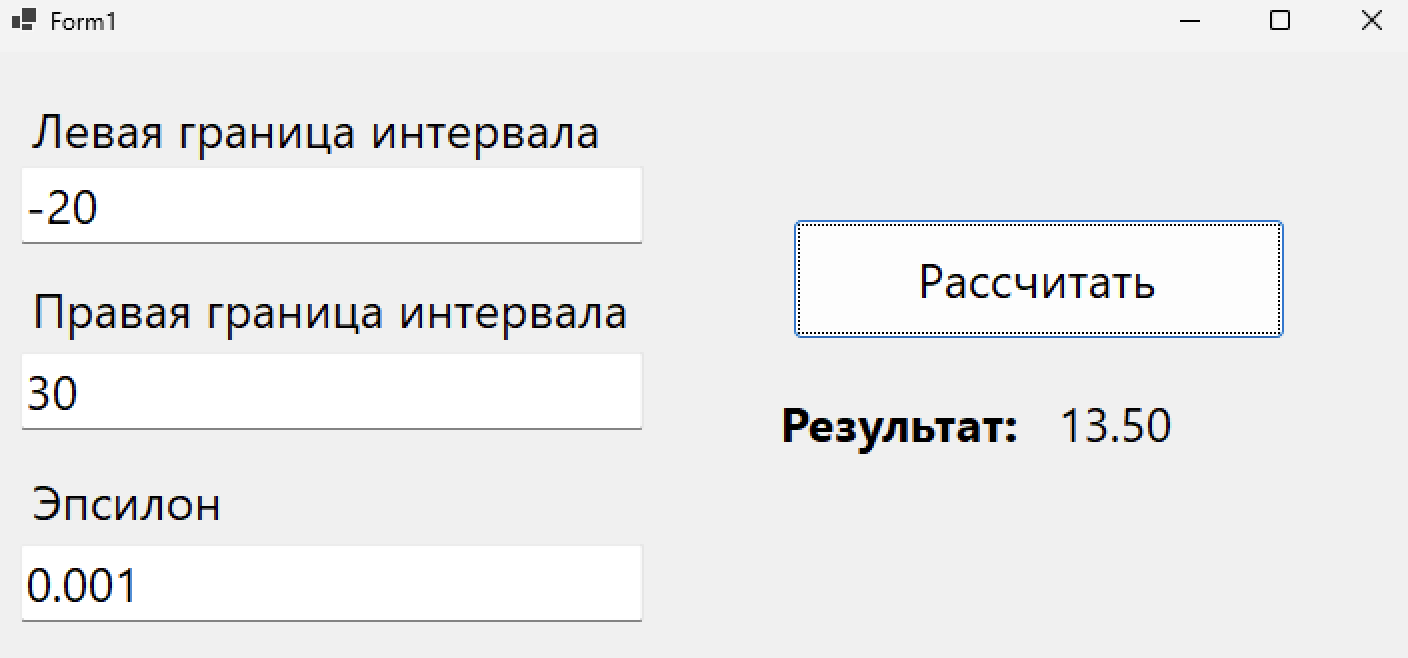
\includegraphics[width=0.7\textwidth]{images/vba/filled-form.png}
  \caption{Результат вычисления}
  \label{fig:vba/filled-form}
\end{figure}

\subsection{Разработка с помощью Delphi}

Для разработки программы на языке программирования Delphi была выбрана среда
разработки Delphi 11 CE от Embarcadero Technologies, поскольку она обладает
обширным инструментарием для создания программ с графическим интерфейсом на
данном языке программирования.

На рисунке \ref{fig:delphi/design} показан дизайн приложения, который был
сделан с помощью средств разработки интерфейсов Delphi 11 CE. В нем есть
поля для ввода границ интервалов, а также точности (эпсилон).

\begin{figure}[H]
  \centering
  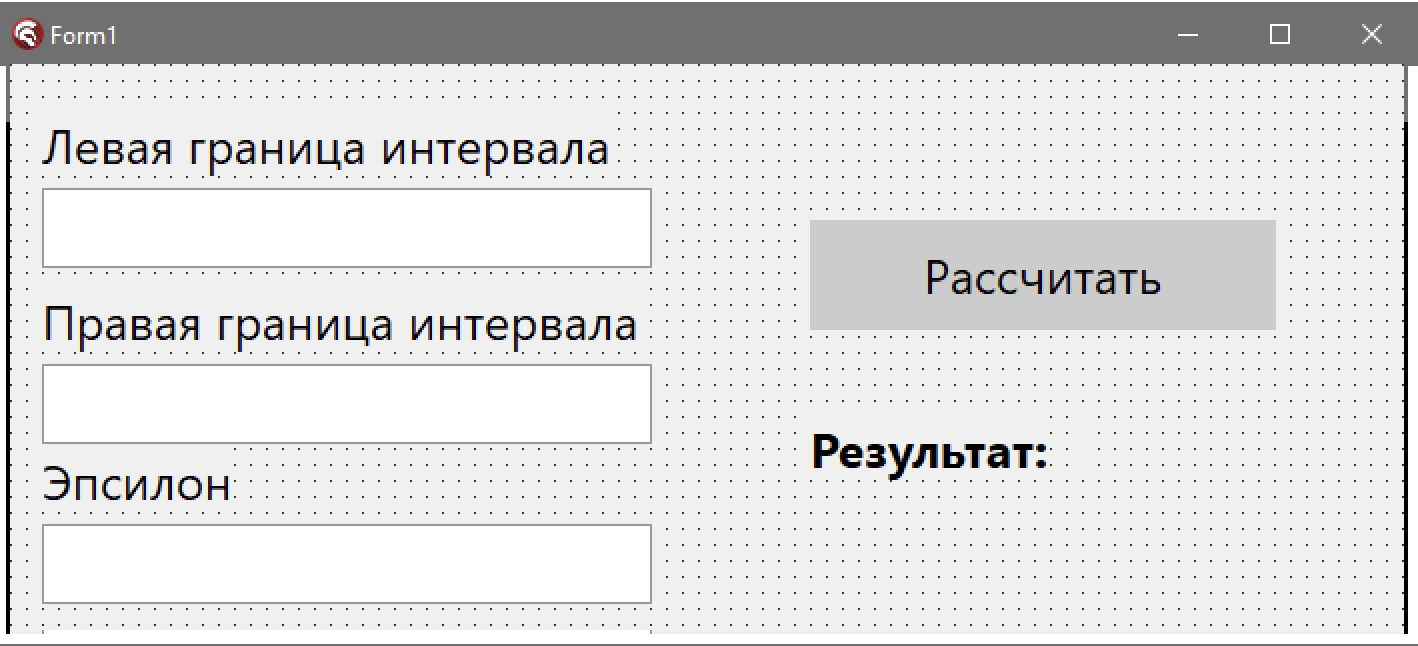
\includegraphics[width=0.7\textwidth]{images/delphi/design.png}
  \caption{Дизайн приложения для вычисления корня уравнения}
  \label{fig:delphi/design}
\end{figure}

При запуске программы открывается окно, показанное на рисунке
\ref{fig:delphi/empty-form}. После ввода данных и нажатия на кнопку <<Рассчитать>>,
как показано на рисунке \ref{fig:delphi/filled-form}, рядом с надписью
<<Результат>> появилось вычисленное значение корня уравнения.

\begin{figure}[H]
  \centering
  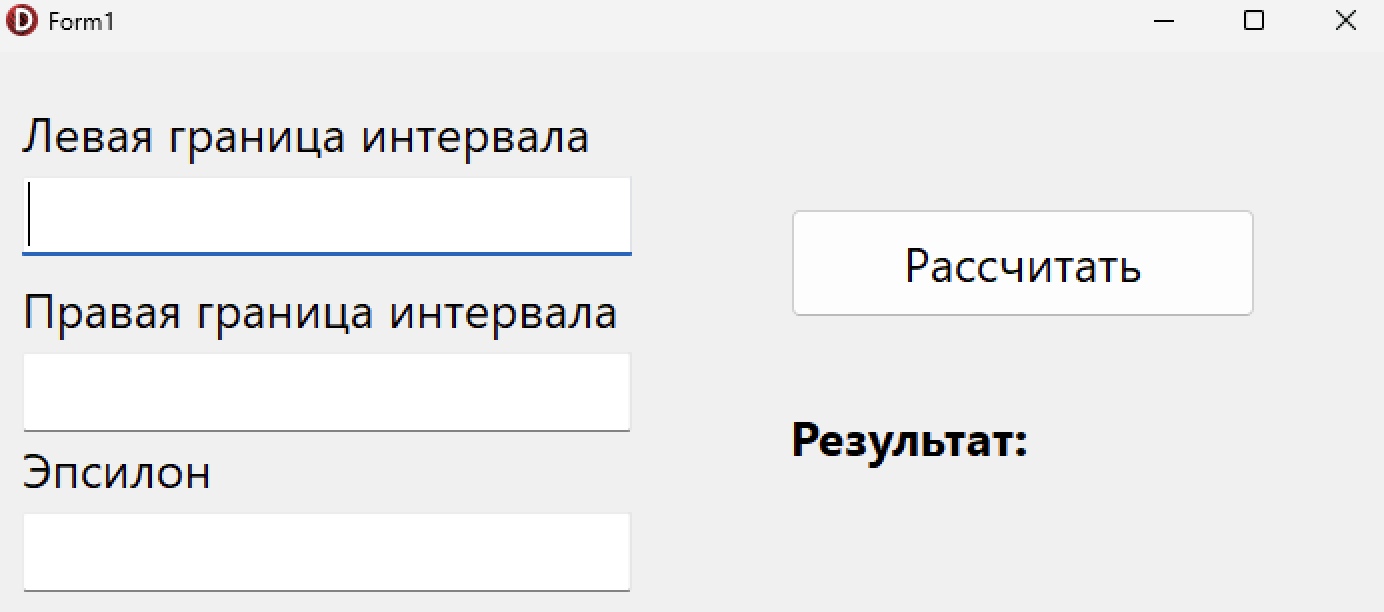
\includegraphics[width=0.7\textwidth]{images/delphi/empty-form.png}
  \caption{Приложение для вычисления корня уравнения}
  \label{fig:delphi/empty-form}
\end{figure}

\begin{figure}[H]
  \centering
  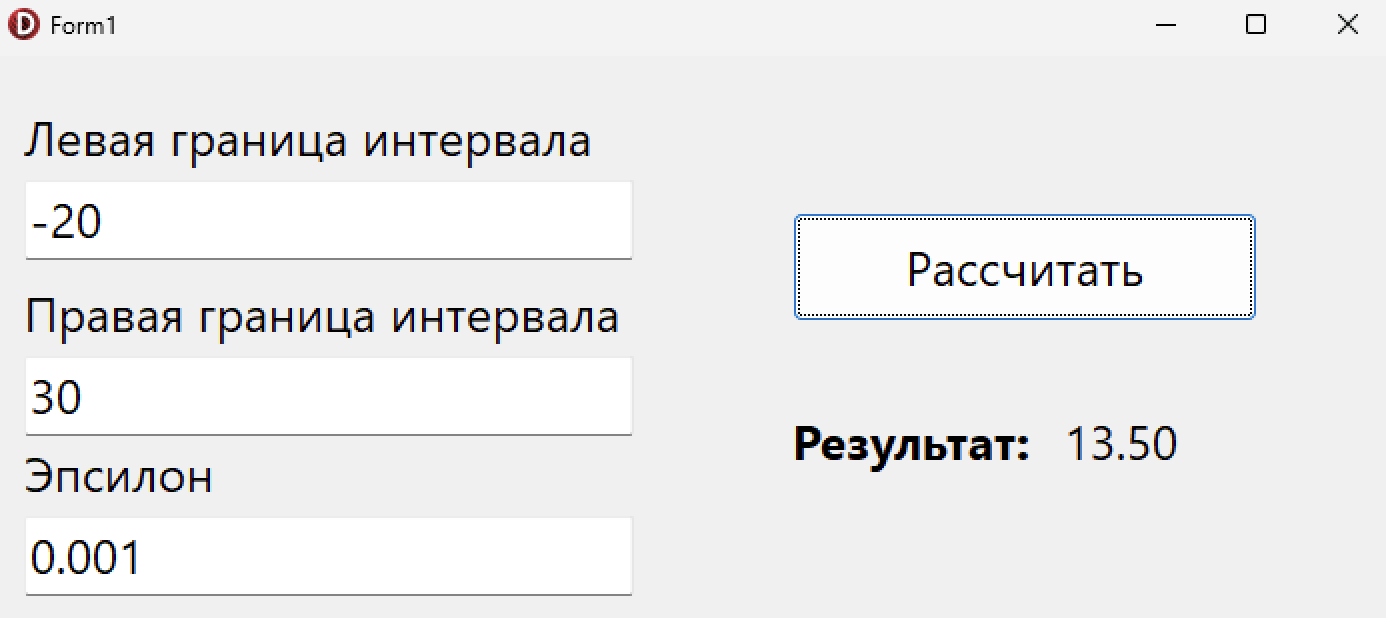
\includegraphics[width=0.7\textwidth]{images/delphi/filled-form.png}
  \caption{Результат вычисления}
  \label{fig:delphi/filled-form}
\end{figure}

\section{Вывод}

В ходе выполнения лабораторной работы было разработано настольное приложение, в
котором у пользователь может получить приближенное решение нелинейного
уравнения с заданной степенью точности.

\end{document}
